\section{Fault Model and Protection Mechanisms}\label{sec:fault}
The evaluation freezes a trained model, its numerical execution and its task data; builds protection assignments from calibration data; and compares them under common random faults (Fig.~\ref{fig:workflow}). All clean and faulted outcomes come from the quantized executable itself, not from the differentiable companion model used to compute gradients. NetSuRF is the software implementation of this workflow; it is not a ranking in the comparison.

\begin{figure}[t]
\centering% Vector adaptation of the original NetSuRF three-panel workflow.
% The historical visual structure is retained; all stages describe software evidence.
\begingroup%
\definecolor{flowbrown}{HTML}{693E25}%
\definecolor{flowcream}{HTML}{FAF6ED}%
\definecolor{flowgreen}{HTML}{EEF3D7}%
\definecolor{flowolive}{HTML}{84944B}%
\definecolor{flowred}{HTML}{B74232}%
\definecolor{flowink}{HTML}{343A3C}%
\resizebox{\linewidth}{!}{%
\begin{tikzpicture}[
  font=\sffamily\fontsize{8}{10}\selectfont,
  text=flowink, >=Stealth,
  edge/.style={->,draw=flowbrown,line width=.75pt},
  transfer/.style={->,draw=flowred,line width=1.15pt},
  group/.style={draw=flowbrown,fill=flowgreen,rounded corners=5pt,
                dashed,line width=.75pt},
  label/.style={align=center,font=\sffamily\bfseries\fontsize{8.3}{10}\selectfont},
  detail/.style={align=center,font=\sffamily\fontsize{7.7}{9.6}\selectfont}]

% Three familiar framed panels and brown stage headers.
\foreach \x in {0,4.6,9.2}{
  \draw[draw=flowbrown,fill=flowcream,line width=.9pt]
    (\x,0) rectangle +(4.4,5.9);
  \fill[flowbrown] (\x,5.12) rectangle +(4.4,.78);
}
\node[align=center,text=white,font=\sffamily\bfseries\fontsize{9.5}{11.5}\selectfont]
  at (2.2,5.51) {1. Frozen network\\and inputs};
\node[align=center,text=white,font=\sffamily\bfseries\fontsize{9.5}{11.5}\selectfont]
  at (6.8,5.51) {2. Stored-bit analysis\\and allocation};
\node[align=center,text=white,font=\sffamily\bfseries\fontsize{9.5}{11.5}\selectfont]
  at (11.4,5.51) {3. Paired reliability\\evaluation};

% Panel 1: immutable model and partition documents.
\draw[draw=flowolive,fill=white,line width=.8pt]
  (.35,3.35)--(.35,4.77)--(1.91,4.77)--(2.11,4.57)
  --(2.11,3.35)--cycle;
\draw[draw=flowolive,line width=.6pt]
  (1.91,4.77)--(1.91,4.57)--(2.11,4.57);
\node[label] at (1.23,4.31) {Frozen INT8\\checkpoint};
\node[detail] at (1.23,3.70) {Stored codes\\Scale / hash};
\draw[draw=flowolive,fill=white,line width=.8pt]
  (2.32,3.35)--(2.32,4.77)--(3.86,4.77)--(4.06,4.57)
  --(4.06,3.35)--cycle;
\draw[draw=flowolive,line width=.6pt]
  (3.86,4.77)--(3.86,4.57)--(4.06,4.57);
\node[label] at (3.19,4.31) {Task inputs};
\node[detail] at (3.19,3.80) {Calibration\\Evaluation};
\draw[group] (.30,.72) rectangle (4.10,2.91);
\node[label,text=flowbrown] at (2.20,2.61) {Verified frozen executable};
\draw[edge] (1.23,3.35)--(1.23,2.91);
\draw[edge] (3.19,3.35)--(3.19,2.91);
% Compact network motif, not a claim about a particular architecture.
\foreach \ya in {1.40,2.04}{
  \foreach \yb in {1.23,1.72,2.21}{
    \draw[flowbrown!45,line width=.45pt] (.65,\ya)--(1.10,\yb);
  }
}
\foreach \ya in {1.23,1.72,2.21}{
  \foreach \yb in {1.40,2.04}{
    \draw[flowbrown!45,line width=.45pt] (1.10,\ya)--(1.55,\yb);
  }
}
\foreach \x/\y in {.65/1.40,.65/2.04,1.10/1.23,1.10/1.72,1.10/2.21,1.55/1.40,1.55/2.04}{
  \filldraw[fill=white,draw=flowbrown,line width=.6pt] (\x,\y) circle (.075);
}
\node[detail,text width=2.10cm] at (2.91,1.73)
  {Exact model bytes\\Pinned backend\\Clean reference};
\node[detail,text=flowbrown] at (2.20,.34) {No retraining or model substitution};

% Panel 2: bit-table stack, calibration group, and sealed-mask motif.
\draw[draw=flowolive,fill=white,line width=.6pt]
  (5.02,3.48) rectangle (6.83,4.88);
\draw[draw=flowolive,fill=white,line width=.6pt]
  (4.94,3.40) rectangle (6.75,4.80);
\draw[draw=flowolive,fill=white,line width=.8pt]
  (4.86,3.32) rectangle (6.67,4.72);
\node[label] at (5.765,4.34) {Bit identities};
\node[detail] at (5.765,3.77) {Tensor / word\\Bit / XOR jump};
\node[label,text=flowbrown] at (7.85,4.70) {Fixed mask $P$};
\foreach \x in {0,...,3}{
  \foreach \y in {0,1}{
    \draw[draw=flowbrown!70,fill=white,line width=.55pt]
      (7.13+\x*.36,3.63+\y*.36) rectangle +(0.36,.36);
  }
}
\foreach \x/\y in {0/1,1/1,2/0}{
  \fill[flowolive!75] (7.13+\x*.36+.025,3.63+\y*.36+.025)
    rectangle +(0.31,.31);
}
\node[detail] at (7.85,3.36) {$|P|=B$};
\draw[group] (4.90,.72) rectangle (8.70,2.91);
\node[label,text=flowbrown] at (6.80,2.60) {Calibrate scores; order bits};
\node[detail] at (6.80,2.12) {Significance $\cdot$ jump $\cdot$ gradients};
\node[detail] at (6.80,1.73) {Published-form FKeras (TFLite)};
\node[label,text=flowred] at (6.80,1.13) {Choose budget; freeze mask};
\draw[edge] (5.765,3.32)--(5.765,2.91);
\draw[edge] (7.85,2.91)--(7.85,3.14);
\draw[transfer] (4.10,1.73)--(4.90,1.73);
\node[detail,text=flowbrown] at (6.80,.34) {Construction data only};

% Panel 3: same proposed field, exact suppressed XOR, inference, and outputs.
\draw[group] (9.50,2.30) rectangle (13.30,4.82);
\node[label,text=flowbrown] at (11.40,4.48) {Shared Bernoulli field $Z$};
\node[detail] at (11.40,4.03) {Suppress $P$; apply XOR on $Z\setminus P$};
\draw[transfer] (8.70,4.03)--(9.50,4.03);
\draw[edge] (11.40,3.80)--(11.40,3.58);
\draw[draw=flowbrown!75,fill=white,rounded corners=2pt,line width=.65pt]
  (9.74,2.56) rectangle (13.06,3.56);
\node[label] at (11.40,3.25) {Quantized inference};
\node[detail] at (11.40,2.83) {Held-out inputs; restore};
% Document motif for task measurements.
\draw[draw=flowolive,fill=white,line width=.55pt]
  (9.61,.48) rectangle (11.40,1.91);
\draw[draw=flowolive,fill=white,line width=.75pt]
  (9.53,.40) rectangle (11.32,1.83);
\node[label,text=flowbrown] at (10.425,1.55) {Task results};
\node[detail,font=\sffamily\fontsize{7.3}{8.5}\selectfont] at (10.425,.95)
  {CE / NLL\\Accuracy\\File ROC-AUC};
\draw[edge] (11.40,2.30)--(11.40,2.10)--(10.425,2.10)--(10.425,1.91);
\draw[edge] (11.40,2.10)--(12.36,2.10)--(12.36,1.91);
% Small illustrative chart: the actual measured curves appear in the results.
\draw[draw=flowbrown,line width=.7pt] (11.75,.74)--(11.75,1.78);
\draw[draw=flowbrown,line width=.7pt] (11.75,.74)--(13.12,.74);
\draw[flowred,line width=1.1pt] (11.84,.87)..controls (12.20,.91) and (12.55,1.63)..(13.04,1.66);
\draw[flowolive,line width=1.1pt] (11.84,.85)..controls (12.41,.86) and (12.73,1.27)..(13.04,1.40);
\node[detail,text=flowbrown] at (12.42,.39) {BER / budget curves};

\node[align=center,font=\sffamily\fontsize{7.6}{9.5}\selectfont,text=flowbrown]
  at (6.80,-.45)
  {Ideal logical suppression $\cdot$ Paired saved fields $\cdot$ Exact restoration $\cdot$ Archived results};
\end{tikzpicture}%
}%
\endgroup%

\caption{Evaluation workflow. A ranking or a rate-aware search fixes which bits are protected and how, and a fault field proposes random flips; the two are separate objects. Assignments are frozen before paired evaluation. Protection cost counts storage bits; physical correction circuits are outside the study.}
\Description{Frozen model and bit identities lead to calibration-based rankings, fixed protection masks, paired exact faults and task-level reliability measurements.}
\label{fig:workflow}
\end{figure}

\paragraph{Eligible population.} The eligible population contains the $N$ bits of the stored INT8 weight codes: convolution and dense kernels in the TFLite models, and the weight matrices of all linear layers in the transformers. Bit $b$ belongs to weight $w(b)$; position zero is least significant and position seven is the sign bit. Zero-valued weights remain eligible. Biases, quantization scales and zero points, input embedding tables, normalization parameters and activations are not faulted (Appendix~\ref{app:implementation}); they are treated as perfectly reliable at no cost, which is an assumption of the study.

\paragraph{Faults.} A fault XORs one stored bit. Flipping bit $b$ alone moves its weight by an exact jump $\Delta_b$: for code $5$ with scale $1/16$, flipping the sign bit gives code $-123$, a jump of $-8$ codes or $-0.5$. In two's complement the jumps of several flipped bits of one word add exactly. A \emph{fault field} proposes a flip at every stored bit independently with probability $p$, the logical bit-error probability. Copies and check bits are stored bits too and fail with the same $p$.

\paragraph{Protection mechanisms and their residual error.} A mechanism $s$ lowers the probability that a data bit is still wrong after voting or decoding to a residual value $\rho_s(p)$, at a cost of $\mathrm{cost}_s$ extra storage bits per data bit (Table~\ref{tab:mechanisms}, Fig.~\ref{fig:residual}). An \emph{assignment} $A$ gives every data bit a mechanism, and bit $b$ then flips with probability $r_b=\rho_{A(b)}(p)$. The paper's earlier masks are the special case of ideal suppression, $\rho=0$. The curves of Table~\ref{tab:mechanisms} follow from counting failure patterns: a majority vote is wrong when most copies flip; a SEC-DED code repairs one error per word, so a data bit stays wrong when another bit of its $n$-bit word also flips; checksum correction (ABFT) repairs one faulty weight per output channel of $G$ weights, so a flipped bit stays wrong when another weight of its channel is faulty.

\begin{table}[t]
\caption{Residual flip probability of a protected data bit and storage cost. Every stored bit, including copies and check bits, flips independently with probability $p$; voters and decoders are ideal. $^*$ABFT: exact for one-weight repair with fault-free checksum words; wrong repairs and checksum faults (Section~\ref{sec:theory-abft}) make a real decoder worse.}\label{tab:mechanisms}
\centering\small
\begin{tabular}{l l l}\toprule
Mechanism $s$ & $\rho_s(p)$ & Extra storage per data bit\\\midrule
None & $p$ & 0\\
Ideal suppression & $0$ & counted as 1\\
Three copies (TMR) & $3p^2-2p^3$ & 2\\
Five copies & $10p^3-15p^4+6p^5$ & 4\\
SEC-DED, $n$-bit word & $p\,[1-(1-p)^{n-1}]\approx(n-1)p^2$ & $(n-d)/d$ for $d$ data bits\\
ABFT$^*$, $G$ weights per channel & $p\,[1-(1-p)^{8(G-1)}]\approx 8(G-1)p^2$ & two checksum words per channel\\\bottomrule
\end{tabular}
\Description{Residual error probabilities and storage costs of six protection mechanisms.}
\end{table}

\begin{figure}[t]
\centering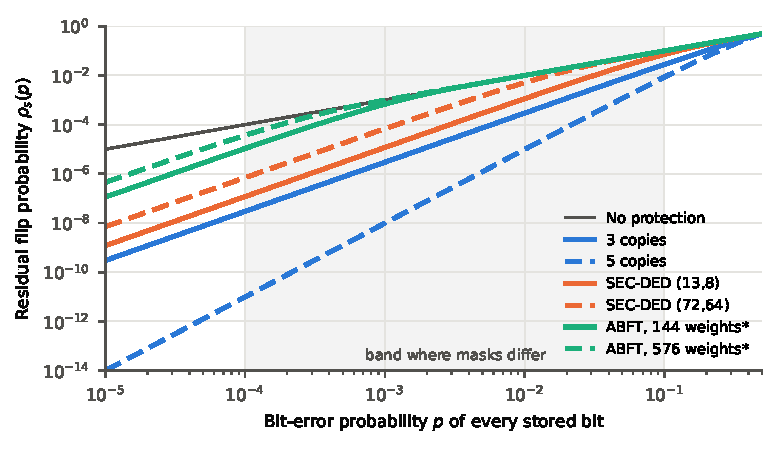
\includegraphics[width=.72\linewidth]{residual_curves}
\caption{Residual flip probability of a protected data bit against the bit-error probability of every stored bit, from Table~\ref{tab:mechanisms}. Copies keep a power law over the whole range. Codes and checksum correction leave it once a second error in the same word or channel becomes likely, near $p\approx1/n$ or $1/(8G)$, and then protect almost nothing. The shaded band is where the masks of this study differ. Curves are analytic; \Branch{R3a}{a bit-level simulation matches every one of them (Section~\ref{sec:mechanisms}).}{\TBD{simulation check outcome}.}}\label{fig:residual}
\Description{Log-log curves of residual error probability for no protection, three and five copies, two SEC-DED codes and two ABFT channel sizes.}
\end{figure}

\paragraph{Why stored weights, and why dense fault rates.} A stored weight is needed for the whole deployment and an activation only until it is consumed, so in the architectural-vulnerability view a weight bit is exposed for much longer~\cite{mukherjee2003avf,deutsch2024delayavf}. On the Eyeriss accelerator the projected failure rate of the filter memory exceeds that of the whole datapath by about three orders of magnitude, although which storage dominates depends on the architecture~\cite{li2017understanding,tyagi2023thales}. Proton tests of ECON-D, a radiation-hard ASIC of the CMS calorimeter upgrade~\cite{cummings2023econd}, combined with the planned luminosity of the High-Luminosity LHC~\cite{hllhc2017tdr}, imply that an unprotected register bit that is never rewritten reaches an upset probability of $10^{-3}$ within hours to days and $10^{-2}$ within days to weeks of beam, the band in which the masks of this study differ. Appendix~\ref{app:faultmotivation} gives the numbers and their limits; neither argument calibrates $p$. Because $p$ grows with the time since the last rewrite, scrubbing moves a deployment along these curves, which is one reason to design for a range of rates rather than for one.
